\section{Regularization and Training}
\label{sec:regularization}

The MPNN was trained with AdamW at learning rate $10^{-3}$ and weight decay
$10^{-5}$, dropout probability 0.2, and a batch size of 64. Training ran for at
most 60 epochs. We selected the checkpoint with the highest mean validation PR
AUC and stopped after 10 epochs without improvement, restoring that checkpoint.
The learning curves in Fig.~\ref{fig:raghav-learning-curves} show training loss
and validation PR AUC for the GCN and MPNN on the scaffold split (seed 0).
Dropout randomly suppresses hidden activations, while AdamW weight decay limits
large parameter values; both are standard controls against overfitting in
small-data neural models \cite{srivastava2014dropout,loshchilov2019decoupled}.

For each endpoint, the positive-class weight was calculated from labeled
training molecules as $n_{\mathrm{neg}}/n_{\mathrm{pos}}$, capped at 50.
Binary cross-entropy was masked so an untested molecule-assay pair contributed
no loss. This matters because missing Tox21 outcomes do not mean inactive.
DropEdge removes a fraction of graph edges during training and tests whether
stochastic neighborhood perturbation improves generalization
\cite{rong2020dropedge}. The frozen MPNN used hidden size 64, three message
passing steps, dropout 0.2, and weight decay $10^{-5}$. Each ablation changed
one setting and used the same scaffold split and seeds 0--2.

Table~\ref{tab:raghav-regularization} reports the mean endpoint PR AUC, averaged
over seeds, with the sample standard deviation across the three seed-level
means. The frozen MPNN baseline scored $0.3069 \pm 0.0180$. Removing class
weights reduced PR AUC to $0.2944 \pm 0.0202$; treating missing labels as
negative reduced it to $0.3002 \pm 0.0041$. These results are consistent with
the intended roles of imbalance correction and label masking, though the
three-seed differences are descriptive rather than a significance claim.
Removing dropout produced $0.3046 \pm 0.0324$, and removing weight decay
produced $0.3078 \pm 0.0225$, both close to baseline relative to seed
variability. DropEdge at rate 0.2 reached $0.3321 \pm 0.0229$. This is the
largest observed mean, but the small number of seeds and overlapping variation
limit the strength of that conclusion.

\begin{figure}[t]
  \centering
  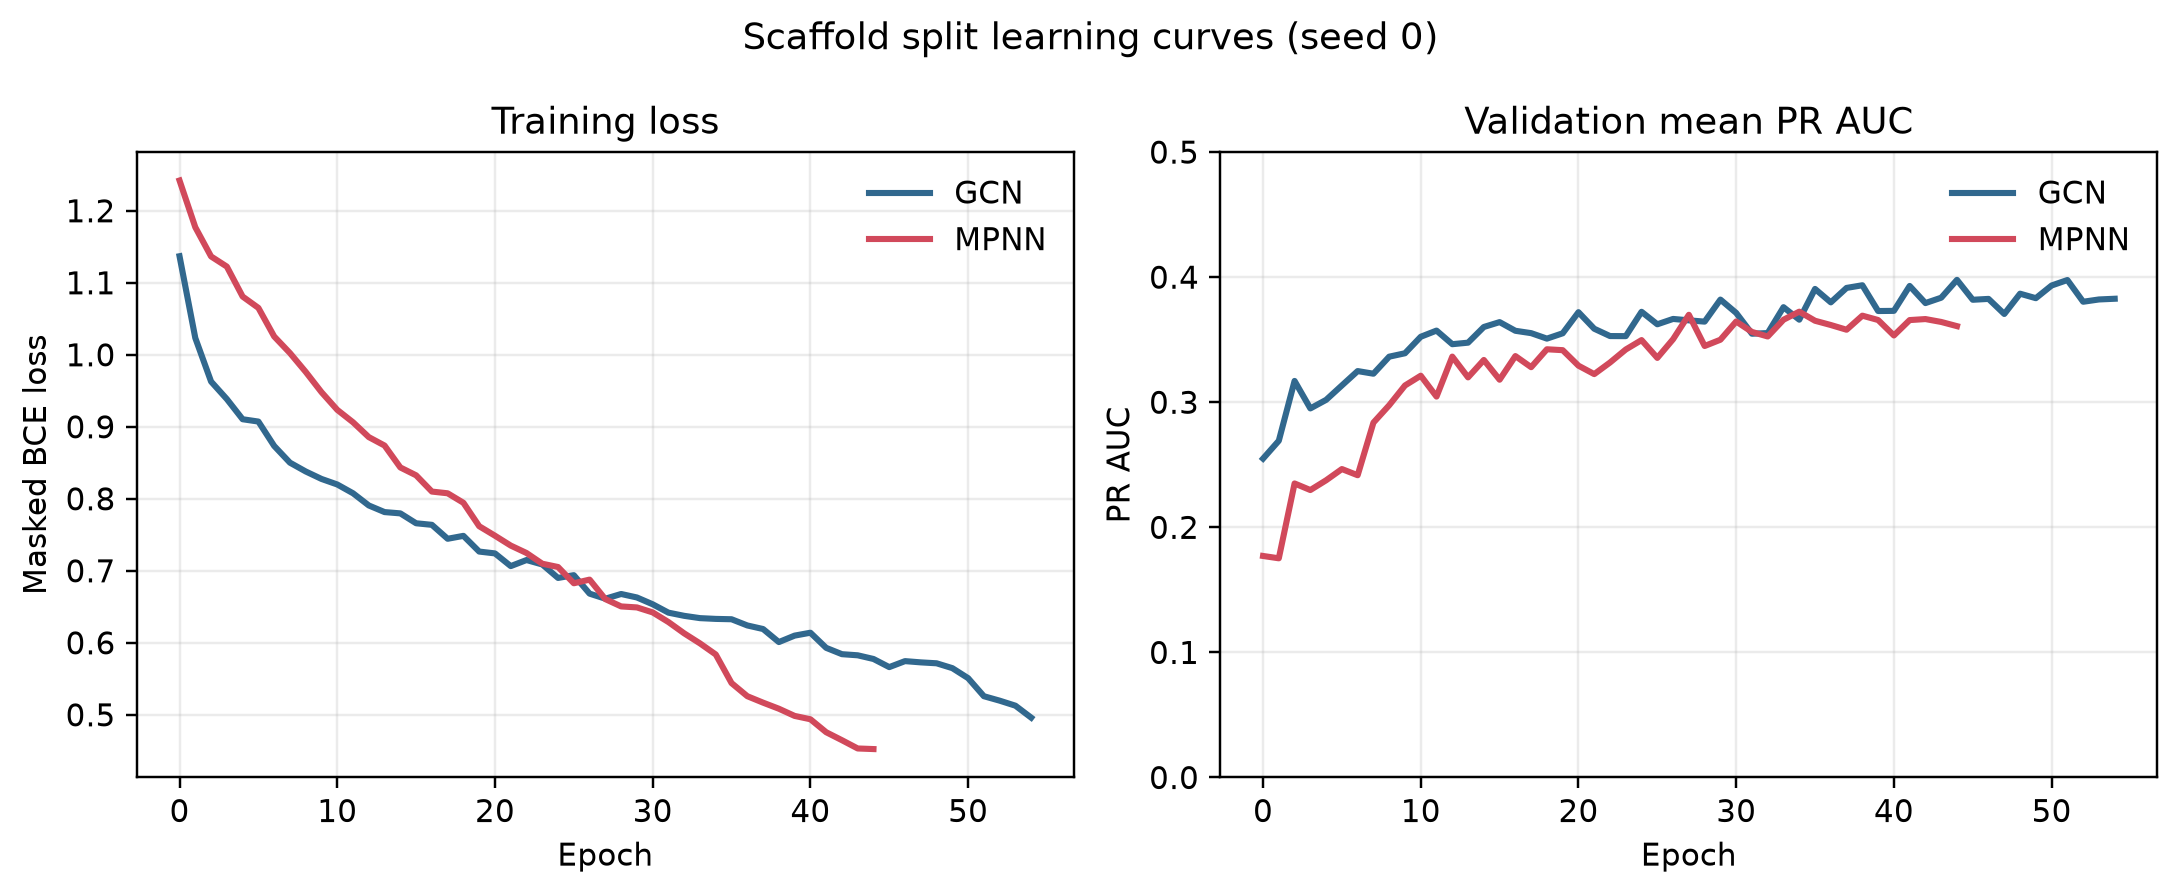
\includegraphics[width=\linewidth]{../figures/raghav_learning_curves.png}
  \caption{Training loss and validation PR AUC for the scaffold split, seed 0.}
  \label{fig:raghav-learning-curves}
\end{figure}

\begin{table}[t]
\centering
\caption{MPNN regularization ablations on the scaffold test split. Values are mean endpoint PR AUC across seeds, mean $\pm$ sample standard deviation across seed-level means.}
\label{tab:raghav-regularization}
\small
\begin{tabular}{lr}
\hline
Setting & PR AUC \\
\hline
Frozen baseline & $0.3069 \pm 0.0180$ \\
No class weights & $0.2944 \pm 0.0202$ \\
No label mask & $0.3002 \pm 0.0041$ \\
No dropout & $0.3046 \pm 0.0324$ \\
No weight decay & $0.3078 \pm 0.0225$ \\
DropEdge ($p=0.2$) & $0.3321 \pm 0.0229$ \\
\hline
\end{tabular}
\end{table}
